\documentclass[tikz,border=7pt]{standalone}
\usepackage[siunitx]{circuitikz}
\usetikzlibrary{calc,arrows.meta}

\definecolor{hptcore}{RGB}{112,112,112}
\definecolor{hptgreen}{RGB}{92,125,58}
\definecolor{hptorange}{RGB}{220,112,32}
\definecolor{hptpurple}{RGB}{128,98,160}

\begin{document}
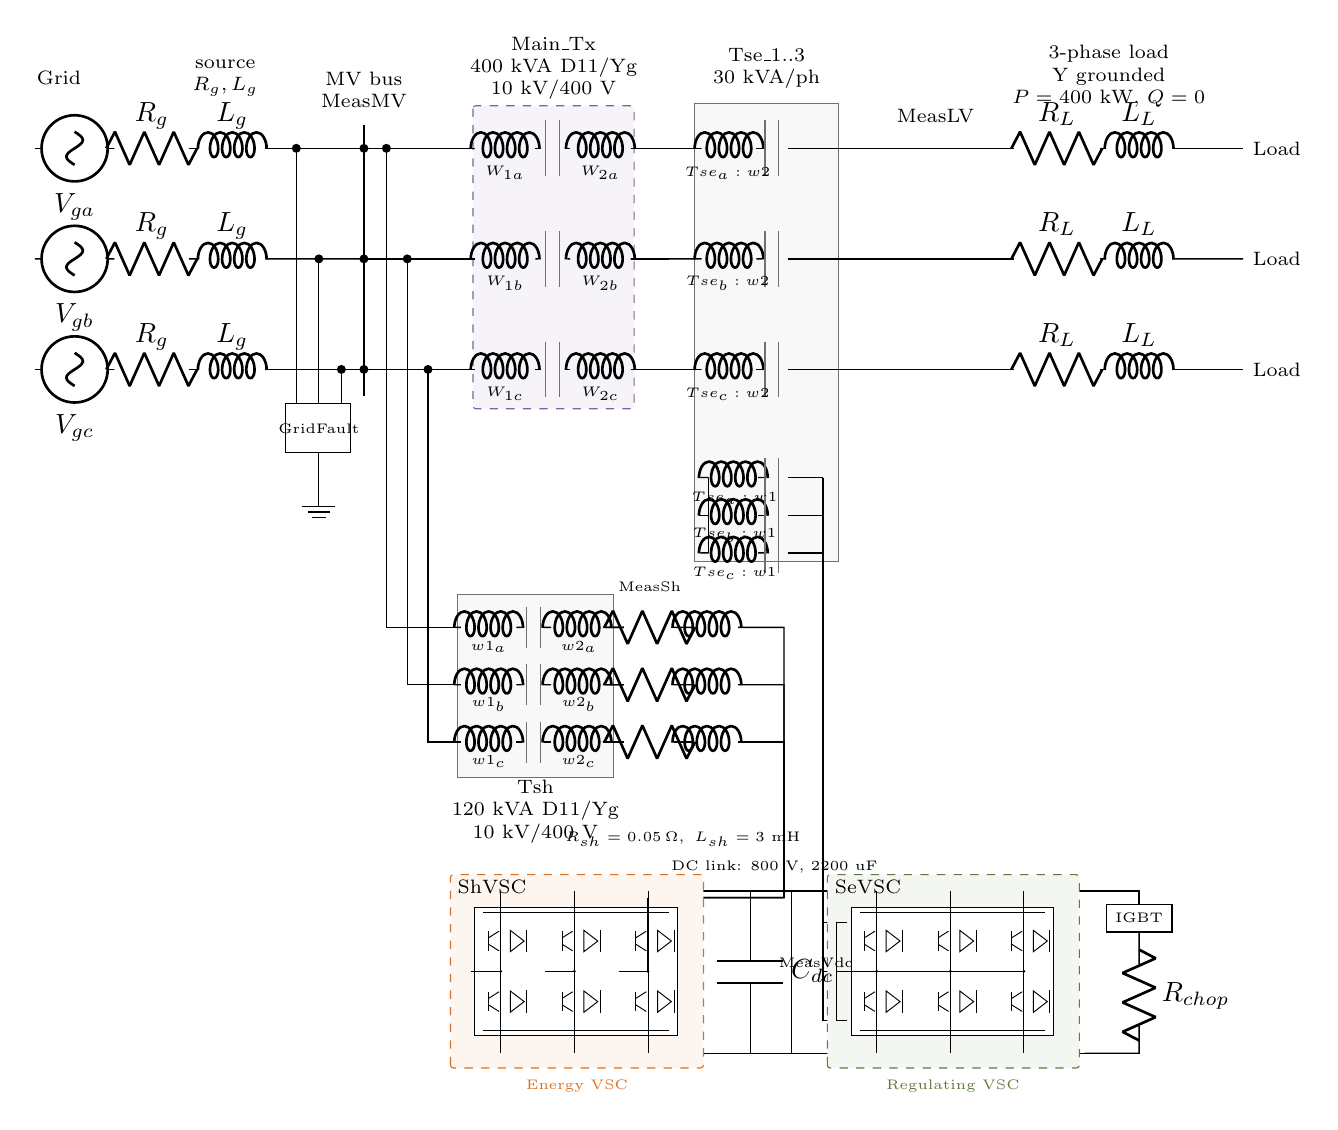
\begin{tikzpicture}[american voltages, x=1.10cm, y=1.04cm]
  \tikzset{
    bus/.style={line width=0.48pt},
    thinbus/.style={line width=0.34pt},
    core/.style={line width=0.42pt, draw=hptcore},
    dot/.style={circle, fill, inner sep=1.15pt},
    terminal/.style={circle, draw, fill=white, inner sep=1.0pt, line width=0.32pt},
    note/.style={font=\scriptsize, align=center},
    tiny/.style={font=\tiny, align=center},
    body/.style={draw=hptcore, fill=hptcore!5, line width=0.36pt},
    conv/.style={draw, fill=white, line width=0.42pt},
    orangebox/.style={draw=hptorange, dashed, fill=hptorange!7, rounded corners=1pt},
    greenbox/.style={draw=hptgreen, dashed, fill=hptgreen!7, rounded corners=1pt},
    purplebox/.style={draw=hptpurple, dashed, fill=hptpurple!7, rounded corners=1pt}
  }

  \newcommand{\igbtswitch}[2]{%
    \draw[thinbus] (#1,#2+0.18) -- (#1,#2-0.18);
    \draw[thinbus] (#1-0.14,#2+0.12) -- (#1-0.14,#2-0.12);
    \draw[thinbus] (#1-0.14,#2+0.04) -- (#1-0.02,#2+0.12);
    \draw[thinbus] (#1-0.14,#2-0.04) -- (#1-0.02,#2-0.12);
    \draw[thinbus] (#1+0.11,#2-0.13) -- (#1+0.27,#2) -- (#1+0.11,#2+0.13) -- cycle;
    \draw[thinbus] (#1+0.30,#2-0.14) -- (#1+0.30,#2+0.14);
  }

  \newcommand{\bridgeleg}[2]{%
    \draw[thinbus] (#1,#2+0.72) -- (#1,#2-0.72);
    \draw[thinbus] (#1-0.34,#2) -- (#1,#2);
    \fill (#1,#2) circle[radius=0.018];
    \igbtswitch{#1}{#2+0.37}
    \igbtswitch{#1}{#2-0.37}
  }

  \newcommand{\phasetx}[5]{%
    \draw[bus] (#1,#2) to[L] (#1+0.70,#2);
    \draw[core] (#1+0.82,#2+0.34) -- (#1+0.82,#2-0.34);
    \draw[core] (#1+0.98,#2+0.34) -- (#1+0.98,#2-0.34);
    \draw[bus] (#1+1.10,#2) to[L] (#1+1.80,#2);
    \node[tiny] at (#1+0.35,#2-0.30) {#3};
    \node[tiny] at (#1+1.45,#2-0.30) {#4};
    \node[tiny] at (#1+0.90,#2+0.48) {#5};
  }

  % ---------------------------------------------------------------------------
  % Grid source with internal weak-grid impedance, MV bus, and MV fault.
  % ---------------------------------------------------------------------------
  \foreach \y/\ph in {3.9/a,2.55/b,1.20/c} {
    \draw[bus] (-0.20,\y) to[sV,l_=$V_{g\ph}$] (0.72,\y)
      to[R,l=$R_g$] (1.58,\y)
      to[L,l=$L_g$] (2.58,\y)
      -- (3.60,\y);
  }
  \node[note] at (0.08,4.76) {Grid};
  \node[note] at (2.00,4.76) {source\\$R_g,L_g$};
  \draw[bus] (3.60,4.18) -- (3.60,0.88);
  \node[note] at (3.60,4.61) {MV bus\\MeasMV};
  \foreach \y in {3.9,2.55,1.20} {
    \node[dot] at (3.60,\y) {};
  }

  \draw[thinbus] (2.70,0.18) rectangle (3.45,0.78);
  \node[tiny] at (3.08,0.48) {GridFault};
  \foreach \srcy/\x in {3.9/2.82,2.55/3.08,1.20/3.34} {
    \node[dot] at (\x,\srcy) {};
    \draw[thinbus] (\x,\srcy) -- (\x,0.78);
  }
  \draw[thinbus] (3.08,0.18) -- ++(0,-0.25) node[ground]{};

  % ---------------------------------------------------------------------------
  % Main transformer, drawn as an electromagnetic body with three phase windings.
  % ---------------------------------------------------------------------------
  \draw[purplebox] (4.86,4.42) rectangle (6.72,0.72);
  \node[note] at (5.79,4.88) {Main\_Tx\\400 kVA D11/Yg\\10 kV/400 V};
  \foreach \y/\ph in {3.9/a,2.55/b,1.20/c} {
    \draw[bus] (3.60,\y) -- (4.88,\y);
    \phasetx{4.88}{\y}{$W_{1\ph}$}{$W_{2\ph}$}{};
    \draw[bus] (6.68,\y) -- (7.12,\y);
  }

  % ---------------------------------------------------------------------------
  % Series injection transformers. Each phase is a real transformer unit:
  % w2 is in series with the LV line, while w1 is fed by SeVSC. No dashed
  % association line is used; both windings sit in the same transformer body.
  % ---------------------------------------------------------------------------
  \draw[body] (7.42,4.45) rectangle (9.08,-1.15);
  \node[note] at (8.25,4.88) {Tse\_1..3\\30 kVA/ph};
  \foreach \y/\ph in {3.9/a,2.55/b,1.20/c} {
    \draw[bus] (7.12,\y) -- (7.50,\y) to[L] (8.13,\y);
    \draw[core] (8.23,\y+0.34) -- (8.23,\y-0.34);
    \draw[core] (8.39,\y+0.34) -- (8.39,\y-0.34);
    \draw[bus] (8.50,\y) -- (11.10,\y);
    \node[tiny] at (7.80,\y-0.30) {$Tse_{\ph}:w2$};
  }
  \foreach \y/\ph/\porty in {-0.12/a/-5.55,-0.58/b/-6.15,-1.04/c/-6.75} {
    \draw[bus] (7.58,\y) to[L] (8.15,\y);
    \draw[core] (8.23,\y+0.24) -- (8.23,\y-0.24);
    \draw[core] (8.39,\y+0.24) -- (8.39,\y-0.24);
    \draw[bus] (8.50,\y) -- (8.90,\y);
    \draw[bus] (8.90,\y) |- (9.18,\porty);
    \node[tiny] at (7.88,\y-0.25) {$Tse_{\ph}:w1$};
  }
  \draw[bus] (7.58,-0.12) -- (7.58,-1.04);

  % LV load.
  \node[note] at (10.20,4.30) {MeasLV};
  \foreach \y in {3.9,2.55,1.20} {
    \draw[bus] (11.10,\y) to[R,l=$R_L$] (12.10,\y) to[L,l=$L_L$] (13.00,\y)
      -- (13.75,\y);
    \node[right,note] at (13.75,\y) {Load};
  }
  \node[note] at (12.20,4.78) {3-phase load\\Y grounded\\$P=400$ kW, $Q=0$};

  % ---------------------------------------------------------------------------
  % Shunt branch: MeasMV -> Tsh primary; Tsh secondary -> MeasSh -> Rsh/Lsh
  % -> ShVSC AC terminals.
  % ---------------------------------------------------------------------------
  \foreach \srcy/\yy/\tapx in {3.9/-1.95/3.86,2.55/-2.65/4.10,1.20/-3.35/4.34} {
    \node[dot] at (\tapx,\srcy) {};
    \draw[bus] (\tapx,\srcy) |- (4.72,\yy);
  }
  \draw[body] (4.68,-1.55) rectangle (6.48,-3.78);
  \node[note] at (5.58,-4.20) {Tsh\\120 kVA D11/Yg\\10 kV/400 V};
  \foreach \yy/\ph in {-1.95/a,-2.65/b,-3.35/c} {
    \draw[bus] (4.72,\yy) to[L] (5.36,\yy);
    \draw[core] (5.48,\yy+0.25) -- (5.48,\yy-0.25);
    \draw[core] (5.64,\yy+0.25) -- (5.64,\yy-0.25);
    \draw[bus] (5.76,\yy) to[L] (6.36,\yy) -- (6.60,\yy);
    \node[tiny] at (5.04,\yy-0.24) {$w1_{\ph}$};
    \node[tiny] at (6.08,\yy-0.24) {$w2_{\ph}$};
  }
  \node[tiny] at (6.90,-1.45) {MeasSh};
  \foreach \yy/\portx in {-1.95/5.18,-2.65/6.03,-3.35/6.88} {
    \draw[bus] (6.60,\yy) to[R] (7.20,\yy) to[L] (7.92,\yy) -- (8.45,\yy)
      |- (\portx,-5.25);
  }
  \node[tiny] at (7.28,-4.54) {$R_{sh}=0.05\,\Omega,\ L_{sh}=3$ mH};

  % ---------------------------------------------------------------------------
  % Shared DC bus and detailed power-electronic bridges.
  % ---------------------------------------------------------------------------
  \coordinate (dcpA) at (4.78,-5.17);
  \coordinate (dcpB) at (11.92,-5.17);
  \coordinate (dcnA) at (4.78,-7.15);
  \coordinate (dcnB) at (11.92,-7.15);
  \draw[bus] (dcpA) -- (dcpB);
  \draw[bus] (dcnA) -- (dcnB);

  \draw[orangebox] (4.60,-7.33) rectangle (7.52,-4.97);
  \node[note] at (5.08,-5.12) {ShVSC};
  \draw[conv] (4.88,-6.93) rectangle (7.22,-5.37);
  \foreach \x in {5.18,6.03,6.88} {
    \bridgeleg{\x}{-6.15}
    \draw[bus] (\x,-5.25) -- (\x,-6.15);
    \draw[thinbus] (\x,-5.43) -- (\x,-5.17);
    \draw[thinbus] (\x,-6.87) -- (\x,-7.15);
  }
  \draw[thinbus] (4.98,-5.43) -- (7.12,-5.43);
  \draw[thinbus] (4.98,-6.87) -- (7.12,-6.87);
  \node[tiny,text=hptorange] at (6.06,-7.55) {Energy VSC};

  \draw[greenbox] (8.95,-7.33) rectangle (11.86,-4.97);
  \node[note] at (9.42,-5.12) {SeVSC};
  \draw[conv] (9.23,-6.93) rectangle (11.56,-5.37);
  \foreach \x/\porty in {9.52/-5.55,10.37/-6.15,11.22/-6.75} {
    \bridgeleg{\x}{-6.15}
    \draw[thinbus] (\x,-5.43) -- (\x,-5.17);
    \draw[thinbus] (\x,-6.87) -- (\x,-7.15);
    \draw[bus] (\x-0.34,-6.15) -- (9.06,-6.15) |- (9.18,\porty);
  }
  \draw[thinbus] (9.33,-5.43) -- (11.46,-5.43);
  \draw[thinbus] (9.33,-6.87) -- (11.46,-6.87);
  \node[tiny,text=hptgreen] at (10.40,-7.55) {Regulating VSC};

  \draw (8.06,-5.17) to[C,l=$C_{dc}$] (8.06,-7.15);
  \node[tiny] at (8.34,-4.88) {DC link: 800 V, 2200 uF};
  \draw[bus] (8.54,-5.17) -- (8.54,-7.15);
  \node[tiny] at (8.82,-6.05) {MeasVdc};

  \node[draw, minimum width=0.48cm, minimum height=0.34cm, font=\tiny] (chop) at (12.55,-5.50) {IGBT};
  \draw[bus] (dcpB) -- (12.55,-5.17) -- (chop.north);
  \draw[bus] (chop.south) -- (12.55,-6.07)
    to[R,l=$R_{chop}$] (12.55,-6.81)
    -- (12.55,-7.15) -- (dcnB);
\end{tikzpicture}
\end{document}
